%% LaTeX2e class for seminar theses
%% sections/content.tex
%% 
%% Karlsruhe Institute of Technology
%% Institute for Program Structures and Data Organization
%% Chair for Software Design and Quality (SDQ)
%%
%% Dr.-Ing. Erik Burger
%% burger@kit.edu
%%
%% Version 1.0, 2018-04-16

\section{Basics}
\label{ch:Basics}

In this chapter the basics needed to understand the changes made in SegWit are being explained. These consist of the way a transaction is built (\autoref{sec:Basics:Transaction}), a short explanation of merkle trees and their use (\autoref{sec:Basics:MerkleTree}), and the problems of bitcoin being the current Blocksize limit (\autoref{sec:Basics:BlocksizeLimit}) and Transaction Malleability (\autoref{sec:Basics:TransactionMalleability}). If you already know these basics you can of course skip straight to the SegWit changes (\autoref{ch:SegWit}).

\subsection{Transaction}
\label{sec:Basics:Transaction}

\begin{figure}[!ht]
    \centering
    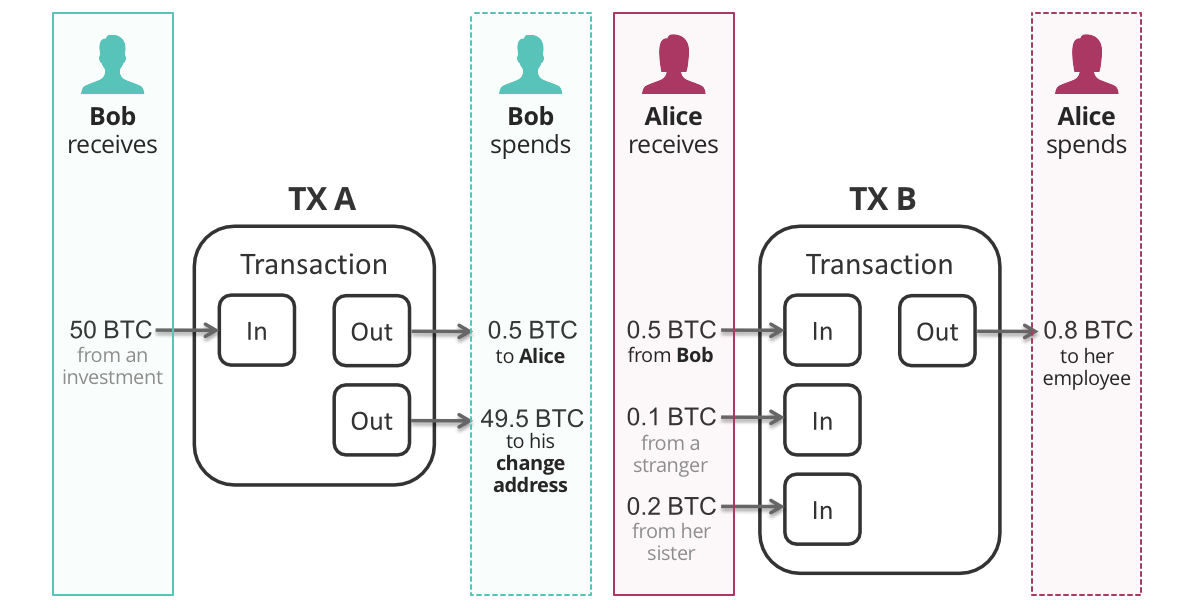
\includegraphics[width=(\textwidth * 2 / 3 )]{Ausarbeitung/images/transaction.png} \caption[Transaction]{Transaction}
    \small \url{https://thecoinrise.com/wp-content/uploads/2019/08/how-do-bitcoin-transaction-work.png}
    \label{fig:transaction}
\end{figure}
Every transaction is built up with a version number, transaction inputs, transaction outputs and a lock time.
The version number just defines which version is used in this transaction. This can be differently for different transactions.
The lock time describes when the transaction should be seen as final. Either it is empty and it should be seen as final on publication, or it has a block height or timestamp as an argument, which tells when the transaction is final.
The first transaction in any block is called "coinbase" transaction and just credits a fix amount of bitcoins plus the sum of all transaction fees in the block. The transaction fees aggregate when the inputs of a transaction contain more bitcoin than the outputs.
Every transaction in any block must have at least one input and at least one output. In \autoref{fig:transaction} Tx A has on Input and two outputs an Tx B has three inputs and one output. The inputs must, except in the "coinbase" transaction, refer to an output of a previous transaction which was not spent yet, called an unspent transaction output or UTXO. For example the first input of Tx B in \autoref{fig:transaction} refers to the first output of Tx A, which is just spent in Tx B.
Finally the transaction has to be signed. There are multiple ways to do this, but the signature is always, before SegWit, contained partly inside the inputs and partly inside the outputs.

\subsubsection{Transaction ID}
To broadcast a transaction into the Bitcoin network it has to be serialized first. Using this serialized data a Transaction ID, or TXID, is calculated for every transaction. This is done by applying double SHA256 on the serialized data and the resulting hash is then used as the ID for this transaction. This is explained further in \autoref{sec:SegWit:Implementation}.


\subsection{Merkle Tree}
\label{sec:Basics:MerkleTree}
\begin{figure}[!ht]
    \centering
    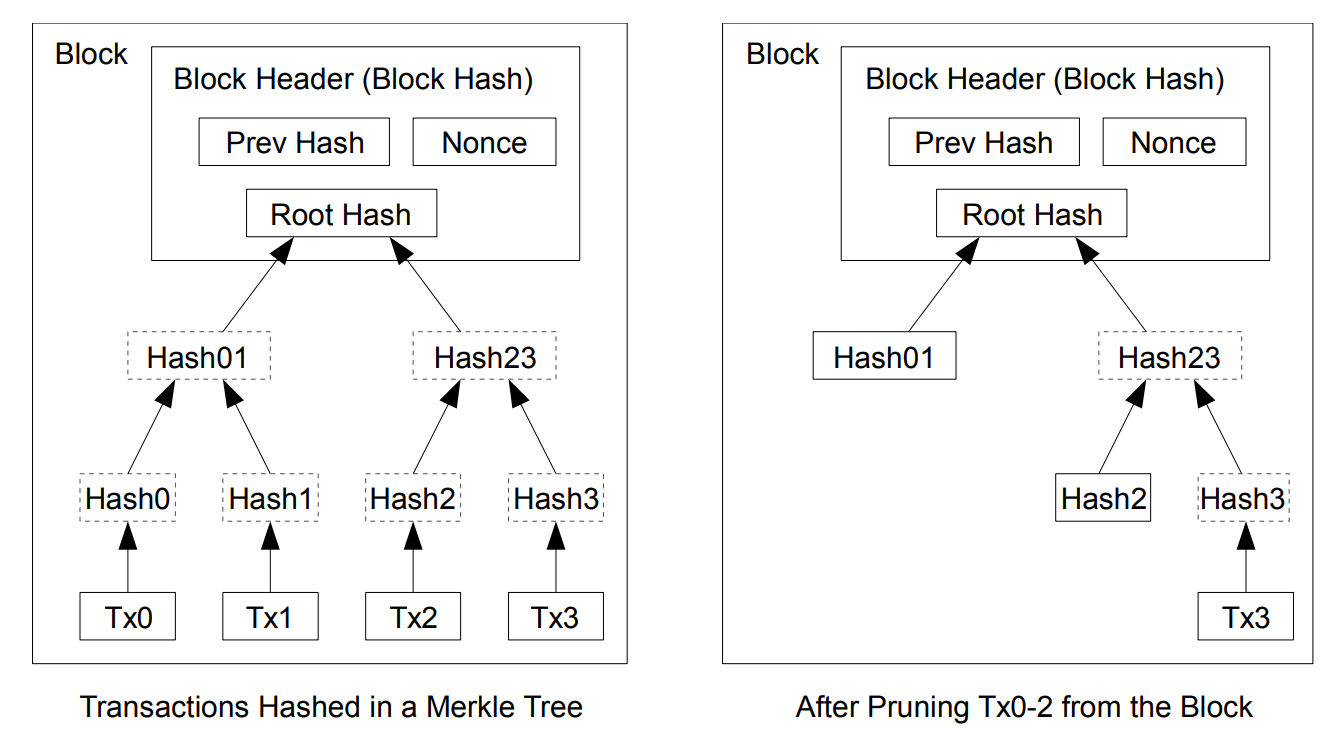
\includegraphics[width=(\textwidth * 2 / 3 )]{Ausarbeitung/images/MerkleTree.png}
    \caption[Merkle Tree]{Merkle Tree}
    \small \url{https://101blockchains.com/wp-content/uploads/2020/05/bitcoin-merkle-transctions.png} 
    \label{fig:merkle_tree}
\end{figure}
A merkle tree, or binary hash tree as shown in \autoref{fig:merkle_tree} is a tree where all the leaves, in the case of bitcoin the leaves are the transactions of a block, are concatenated and then hashed pairwise. This results in a new layer of nodes, which are then again concatenated pairwise and then hashed until there is only one node left, called the merkle root. In \autoref{fig:merkle_tree} the merkle root is called "root hash" and is stored inside the block header, while Tx0 through Tx3 represent the leaves and thus transactions of the corresponding block. As previously described, these transactions are first hashed, resulting in Hash0 through Hash3. Then they are concatenated pairwise and hashed resulting in Hash01 and Hash23. Repeating this process once more this results in the Root Hash. 

The advantage of having a merkle tree is being able to verify quickly if for example Tx3 is contained inside of the block. To do so it is no longer needed to request all transactions of this block by a full bitcoin node, but rather just Hash 2 and Hash01. Of course the block header should be stored locally. To verify if Tx3 is stored inside of this block you need to just calculate Hash3 and together witch Hash2 calculate Hash23 and finally using Hash01 calculate the Root Hash. If this is the same as your locally stored Root Hash you can be sure to assume the transaction (here Tx3) is inside of this block. A more graphic representation of this example can be seen in \autoref{fig:merkle_tree}.



\subsection{Blocksize limit}
\label{sec:Basics:BlocksizeLimit}
Before SegWit blocks were "limited to 1,000,000 bytes (1MB) total size" \cite{bip-141}. This and the fact that there is only supposed to be one new block ever ten minutes \cite{nakamoto} results in an average of about 4.6 transactions per second\footnote{can be seen on \url{https://www.blockchain.com/charts/transactions-per-second}} \cite{hackernoon}.
The theoretical limit can be calculated and is 27 transactions per second \cite{transaction_limit}. But to achieve these 27 transactions per second you have to only use minimal transactions.
Compared to Visa's 1,700 transactions per second \cite{hackernoon} it is obvious that at this state Bitcoin cannot work on a large scale as it simply cannot handle enough transactions.

An important note is, that most of the space inside of a transaction is used up by its signature data. How this is used as an advantage will be discussed in \autoref{sec:SegWit:Implementation}.



\subsection{Transaction Malleability}
\label{sec:Basics:TransactionMalleability}
Since the Transaction ID is calculated by hashing the serialized data of a transaction it is influenced by the signature. There is a problem with this where an attacker can change the whole Transaction ID by changing the unlocking script in a way that does not change the way it works. For example he can just zero pad some data being used which does not change the functionality but very much changes the resulting hash.

\subsubsection{Example of a Malleability attack}
\label{subsec:Basics:TransactionMalleability:Attack}
In this example Alice is the victim and Bob is the attacker.
Alice sends a transaction worth one bitcoin to Bob with Transaction ID A.
Bob now alters the Transaction ID abusing Transaction Malleability and broadcasts the same transaction but with the now different Transaction ID B.
Now Bob is lucky as the transaction with ID B is confirmed before the one with ID A is. Since the UTXO used as input in both transactions is the same, the transaction with Transaction ID A is being declined.
Now Bob, who has received one bitcoin, informs Alice that he has not received the transaction. After Alice checks that no transaction with Transaction ID A got accepted in any block she assumes it must have failed.
Now Alice sends the transaction again resulting in a double spend where Bob receives two bitcoin instead of one.

\subsubsection{Mt.Gox}
One of the biggest bitcoin exchange points ever, which in February 2014 "still accounted for close to 70\% of all bitcoins ever traded" \cite{springer:malleability_and_mtgox}, had to file for bankruptcy in the same month resulting in "the loss of over 500 million USD worth of bitcoins owned by its customers" \cite{springer:malleability_and_mtgox}. \\
Later they stated that the main cause for this was Transaction Malleability \cite{springer:malleability_and_mtgox}.

\subsection{Soft Fork}
\label{sec:Basics:SoftFork}
\begin{figure}[!ht]
    \centering
    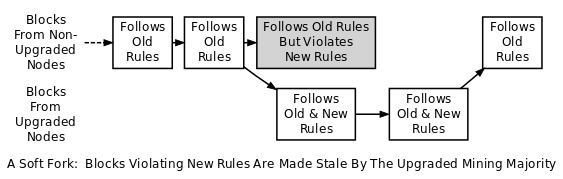
\includegraphics[width=(\textwidth * 2 / 3 )]{Ausarbeitung/images/Softfork.png}
    \caption[Soft Fork]{Soft Fork}
    \small \url{https://wiki.trezor.io/images/Softfork.png} 
    \label{fig:soft_fork}
\end{figure}
To avoid a split in the block chain like a hard fork does, a soft fork still fulfills the old rules used before the update. This way old nodes will still accept transactions following the new rules, because they still have to fulfill the old rules, as seen in \autoref{fig:soft_fork}, but the new nodes do not necessarily accept old transactions.
Thus there is no downside to updating, but at the same time it is not necessary to do so. In the special case of SegWit old transactions will still be valid, this will be further explained in \autoref{sec:SegWit:Idea}.


\section{Segregated Witness}
\label{ch:SegWit}
\todo{description of what segwit is}


\subsection{Idea}
\label{sec:SegWit:Idea}
\begin{figure}[!ht]
    \centering
    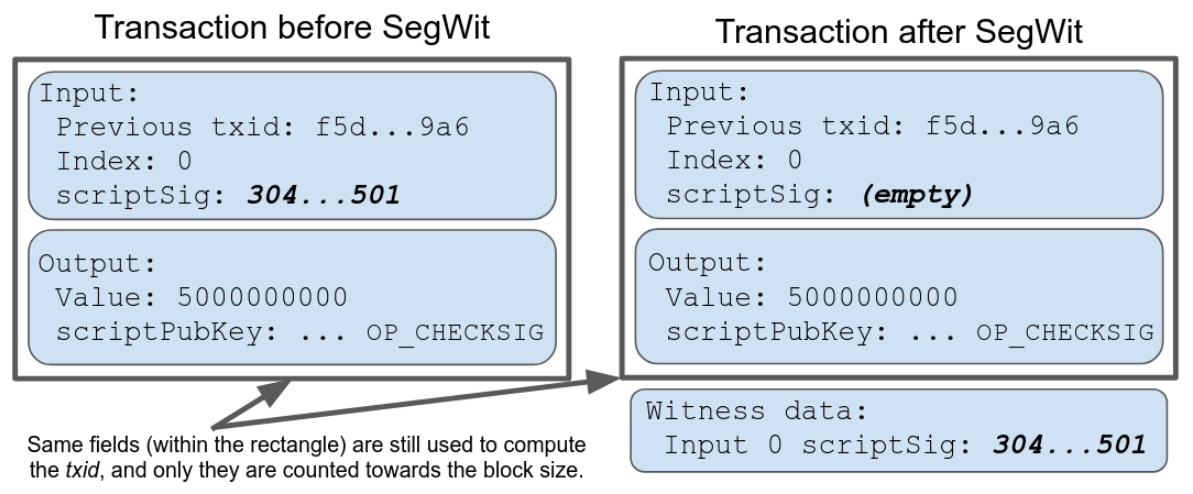
\includegraphics[width=(\textwidth * 2 / 3 )]{Ausarbeitung/images/SegWitTransactionChanges.png}
    \caption[Witness Data]{Witness Data}
    \small \url{https://www.buybitcoinworldwide.com/pages/info/img/segwit-v-legacy.png} 
    \label{fig:segwit_transaction}
\end{figure}
To solve the problem of Transaction Malleability the signature and unlocking script are moved into a new data structure called "witness". This way the signature will no longer affect the identification of a transaction, fixing the problem of Transaction Malleability. In \autoref{fig:segwit_transaction} you can see, that the \textit{scriptSig} in the original transaction block is now empty and the \textit{scriptSig} of the corresponding input is moved into the new witness structure. This new structure has its own ID called WTXID or Witness Transaction Identifier. The separation of witness data from transaction data makes the transmission of the signature data optional, as it is only used for verification of a transaction and not needed for checking its existence.

Additionaly it is implemented in such a way that it is backward compatible, meaning older versions of the Bitcoin protocol are still compatible with these new changes, and can be published as a soft fork, taking away the downside of splitting the network in two. This can be accomplished even though there are many changes made, including an upgrade of the blocksize limit up to theoretical four megabytes. Also Segregated Witness introduces a new commitment structure making future updates simpler.

Finally the fix of Transaction Malleability "allows creation of unconfirmed transaction dependency chains without counterparty risk" \cite{bip-141} like the Lightning network, providing Bitcoin to be a tool for everyday transactions. This has the potential to not only fix Transaction Malleability, but also move a big step to solve the Scalability Problem.


\subsection{Implementation}
\label{sec:SegWit:Implementation}

\begin{figure}[!ht]
    \centering
    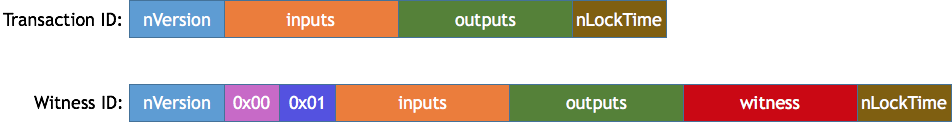
\includegraphics[width=(\textwidth * 2 / 3 )]{Ausarbeitung/images/witnesstxid.png}
    \caption[Calculation of TXID and WTXID]{Calculation of TXID and WTXID}
    \small \url{https://raw.githubusercontent.com/bitcoin/bips/master/bip-0144/witnesstx.png} 
    \label{fig:transaction_ids}
\end{figure}
To implement the new witness we need to define what belongs to this structure. 
To begin with nVersion marks as the name says the version of SegWit. The current version is version zero and all of the following changes, especially witness programs in \autoref{subsec:SegWit:Implementation:WitnessPrograms}, will refer to version zero. The versions one to sixteen are reserved for future updates and there is no further interpretation of the witness program or the witness stack defined yet.
After the version there is a marker which must be a one-byte zero value, as you can see in \autoref{fig:transaction_ids}. "The marker byte is set to zero so that this structure will never parse as a valid transaction in a parser that does not support this BIP" \cite{bip-144}. Not having the marker byte "would lead to empty transactions (no inputs, no outputs, which are used in some tests) to be interpreted as new serialized data" \cite{bip-144}. This of course would lead to errors.
Thirdly the flag byte must be a one byte non-zero value. "Currently, 0x01 MUST be used" \cite{bip-141}. This flag "can be interpreted as a bitvector" \cite{bip-144} and provides space for future extensions to differentiate between witness types.
After the flag come the transaction inputs, each "associated with a witness field" \cite{bip-141}. The count of these is defined by the variable txin\_count. The number of script\_witnesses is thus also implied by the txin\_count. If a transaction is a non-witness transaction it must have an one byte zero value as its associated witness field. The inputs used for calculating the Transaction ID are the same used for calculating the witness ID. 
Same goes for the outputs used for the calculations. The outputs of course show how much of the inputs should be sent to whom.
Probably the most interesting part, the witness part you can see in \autoref{fig:transaction_ids}, will mostly be explained later, as it is more complicated than the rest.
Finally the last part used to calculate the Witness ID is nLockTime, which is the same as described in \autoref{sec:Basics:Transaction}. It is there if you do want the changes to be committed to the block chain at a certain point in the future.

\subsubsection{Witness Root Hash}
\label{subsec:SegWit:Implementation:WitnessRootHash}
To provide the same benefits of a merkle tree, as mentioned in \autoref{sec:Basics:MerkleTree}, to the new witness structure it gets its own merkle tree.
\begin{figure}[!ht]
    \centering
    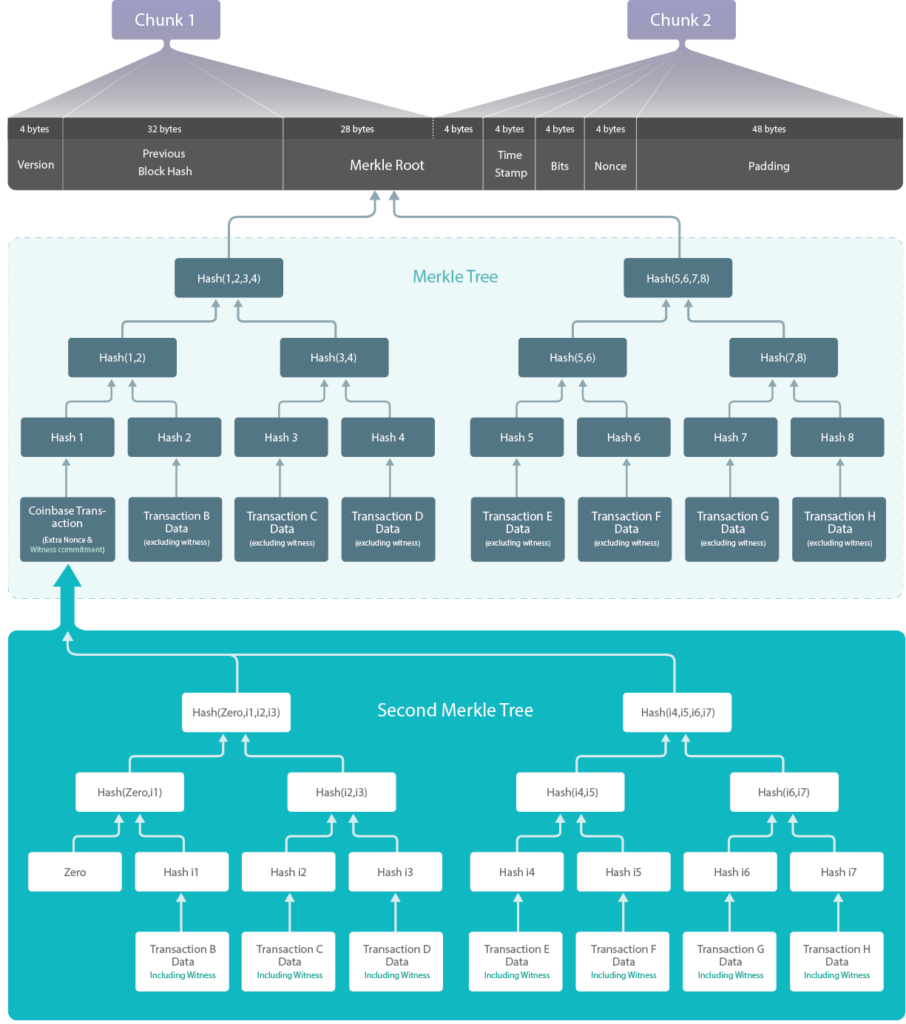
\includegraphics[width=(\textwidth * 2 / 3 )]{Ausarbeitung/images/SegWitMerkleTree.png}
    \caption[Witness Merkle Tree]{Witness Merkle Tree}
    \small \url{https://blog.bitmex.com/wp-content/uploads/2020/01/ASICBOOST_Allegation5-906x1024.png} 
    \label{fig:segwit_merkle_tree}
\end{figure}
This tree is built like the normal merkle tree, but has the Witness IDs defined in \autoref{sec:SegWit:Implementation}, rather than just the Transaction IDs, as its leaves. As the coinbase transaction does not have witness data, its Witness ID "is assumed to be 0x0000....0000" \cite{bip-141}, or in other words is zero.
As you can see in \autoref{fig:segwit_merkle_tree} the resulting witness root hash is not saved in the block header. That is the case, because changes to the block header would remove the ability to publish this update as a soft fork. Instead the witness root hash is stored inside a new structure named commitment structure, which has its place inside of the coinbase transaction.

\subsubsection{Commitment Structure}
\label{subsec:SegWit:Implementation:CommitmentStructure}
The new commitment "is recorded in a \textit{scriptPubKey} of the coinbase transaction" \cite{bip-141} and must be at least 38 bytes and is defined as in \autoref{fig:commitment_structure}.
\begin{figure}[!ht]
    \centering
    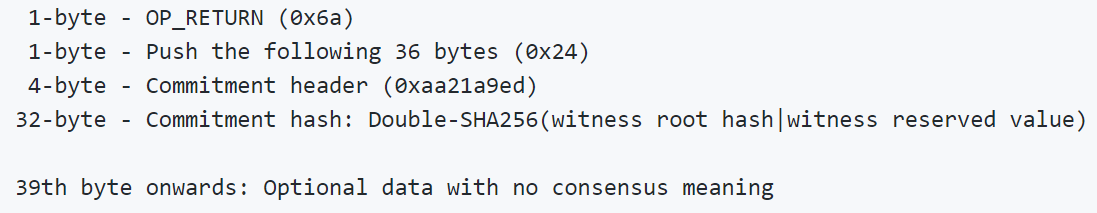
\includegraphics[width=(\textwidth * 2 / 3 )]{Ausarbeitung/images/CommitmentStructure.png}
    \caption[Commitment Structure]{Commitment Structure}
    \small \url{https://github.com/bitcoin/bips/blob/master/bip-0141.mediawiki} 
    \label{fig:commitment_structure}
\end{figure}
The first six byte must be 0x6a24aa21a9ed \cite{bip-141}. The following 32 bytes are the result of hashing a new witness reserved value concatenated to the witness root hash. This new witness reserved value "currently has no consensus meaning, but in the future allows new commitment values for future softforks" \cite{bip-141}. Also if there are multiple \textit{scriptPubKey}s matching this pattern then the \textit{scriptPubKey} with the highest output index is considered as the commitment, although it should rarely happen that multiple \textit{scriptPubKey}s match this pattern.


\subsubsection{Witness Programs}
\label{subsec:SegWit:Implementation:WitnessPrograms}
A new program to handle witness data is introduced in BIP-141. This program is triggered if \textit{scriptPubKey} is a script that consists of firstly a one byte push opcode, called the 'version byte', and then a two to forty byte data push, called the 'witness program'. Also a new validation logic is introduced with two ways to trigger it:
\begin{enumerate}
    \item The \textit{scriptPubKey} has to be exactly a push of a version byte and after that a push of the witness program. Meanwhile the \textit{scriptSig} has to be empty. This is called 'native witness program'.
    \item The \textit{scriptPubKey} has to be a P2SH script (as defined in BIP-16). The belonging \textit{redeem script} has to be a push of a version byte plus a push of a witness program. Additionaly the \textit{redeem script} must be pushed into the \textit{scriptSig}.
\end{enumerate}

In the following only the witness programs with version zero defined in BIP-141 are going to be discussed. The first one is called 'pay-to-witness-public-key-hash' (P2WPKH) while the second is called 'pay-to-witness-script-hash' (P2WSH). To begin with P2WPKH
\begin{itemize}
    \item the version byte must be zero and the witness program must be 20 bytes,
    \item the witness must have exactly two contents, first the signature and then the public key, where both of these have to be at max 520 bytes each,
    \item the witness program must be the HASH160 of the public key,
    \item and if the script is correct, "the signature is verified against the public key with CHECKSIG operation" \cite{bip-141}.
\end{itemize}

For example this is how a version zero native P2WPKH has to look:
\begin{itemize}
    \item witness: <signature> <pubkey>
    \item scriptSig: (empty)
    \item scriptPubKey: <version: 0> <HASH160 of pubkey> \cite{bip-141}
\end{itemize}
The signature is then verified as <signature> <pubkey> CHECKSIG.

Secondly for P2WSH
\begin{itemize}
    \item the version byte must be zero and the witness program must be 32 bytes,
    \item the witness must consist of an input stack for the following script and secondly a serialized script, called 'witnessScript', which has a size limit of 10000 bytes,
    \item and the witness program must be the SHA256 hash of this witnessSript.
\end{itemize}
the witnessScript is then popped off the stack, deserialized and executed with the remaining stack. This must result in a single TRUE on the stack. For example this is how a version zero native P2WPKH might look (here the witnessScript is an one-of-two multi-signature):
\begin{itemize}
    \item witness: 0 <signature1> <1 <pubkey1> <pubkey2> 2 CHECKMULTISIG>
    \item scriptSig: (empty)
    \item scriptPubKey: <version: 0> <SHA256 hash of witnessScript> \cite{bip-141}
\end{itemize}
the witnessScript (1 <pubkey1> <pubkey2> 2 CHECKMULTISIG) is then popped off and its SHA256 hash compared against the witness program. Afterwards it is deserialiced and executed with the remaining stack inside the witness: 0 <signature1> 1 <pubkey1> <pubkey2> 2 CHECKMULTISIG \cite{bip-141}.

If the version byte is set to zero, but the length of the witness program is neither equal to 20-bytes nor to 32-bytes, the script will fail. But if the second data push, here considered to be the witness program, is longer than 40 bytes it will no longer be assumed to be and witness program and thus will pass.

\subsubsection{Block Weight}
\label{subsec:SegWit:Implementation:BlockWeight}
Another big problem that is tried to be solved by SegWit is the scalability problem. As mentioned in \autoref{sec:Basics:BlocksizeLimit} the blocks were limited to 1MB and thus could not handle more than a maximum of 27 transactions per second \cite{transaction_limit}. One way to increase this limit is to raise the blocksize limit. To do so, a new rule using 'block weight' is defined. To calculate the block weight the 'base size' and the 'total size' are needed. The base size is the sum of all serialized data inside a block needed to calculate the Transaction ID and the total size is the sum of all serialized data inside a block needed to calculate the Witness ID. This also includes the data used to calculate the base size. The serialized data needed to calculate these can be seen in \autoref{fig:transaction_ids}. The formula used to calculate the block weight is defined as
\begin{equation*}
    3 * base size + 1 * total size = block weight.
\end{equation*}
The new rule added is \textit{block weight $\leq$ 4,000,000 bytes}.
If a block does not have any SegWit transactions the base size is equal to the total size meaning the formula would be $4 * base size = block weight$ and would result in the old rule that the block cannot be larger than 1MB. So again this change is backward compatible, making a soft fork possible. This change is not just backward compatible, but also makes it possible to have blocks of almost four times the old size of 1MB, as a block which has almost all of its contents inside the witness block has the rule to be at maximum the size of four megabytes. This will of course require very weird transactions, where most data is inside of the witness. But with normal transactions "[t]he average SegWit block size will be roughly 2MB" \cite{segwit_transaction_limit}.

\subsubsection{Sigop Limit}
\label{subsec:SegWit:Implementation:SigopLimit}
The number of sigops in each block "is currently limited to 20,000" \cite{bip-141}. Similar to the introduction of block weight discussed in \autoref{subsec:SegWit:Implementation:BlockWeight} the old limit is "quadrupled to $\leq$ 80,000" \cite{bip-141} and the sigops that can be used before segwit, namely "the current pubkey script, signature script, and P2SH check script are counted at 4 times their previous value" \cite{bip-141}. Again for old nodes the limit is not affected, as the number of sigops they can see will not surpass 20,000. To still raise the limit for new nodes every "P2WPKH input is counted as 1 sigop" \cite{bip-141} and every opcode inside of a P2WSH script will be counted like it was before SegWit. So every CHECKSIG is counted once and "CHECKMULTISIG is counted as 1 to 20 sigops according to the arguments" \cite{bip-141}.


\subsection{Consequences}
\label{sec:SegWit:Consequences}
As already mentioned in \autoref{sec:SegWit:Idea} the main problem fixed by Segregated Witness is Transaction Malleability. It is no longer possible for a third party to create a duplicate of a transaction with another ID. Also SegWit takes a shot at fixing the scalability problem directly by raising the technical block size. The problem is that this is not a solution to the problem but rather a slight improvement as it just raises the blocksize limit by a static value and does not give Bitcoin a way to scale into the future.

\subsection{Future possibilities}
\label{sec:SegWit:Future}
A nice side effect to fixing Transaction Malleability is that it "enables the building of unconfirmed transaction dependency chains in a trust-free manner" \cite{bip-141}. This allows for a new technology to work with bitcoin called the 'Lightning Network'. This new technology could solely fix the scalability problem as it is an off-chain solution that could be able to process up to one million transactions per second. 
\todo{Trust-free unconfirmed transaction dependency chain (Lightning Network), Future extensions}

\subsection{History of Segregated Witness}
\label{sec:SegWit:History}

\todo{find good source for this}
